% !TeX program = lualatex
% !TeX encoding = utf8
% !TeX spellcheck = uk_UA
% !BIB program = bibtex8

\documentclass[]{beamer}
\usetheme{QuantumChemistry}
\usepackage{QuantumChemistry}

\title[Лекції з квантової хімії]{{\huge\bfseries Квантова механіка молекул}\\ Наближення Борна-Оппенгеймера}
\subtitle{Лекції з квантової хімії}
\date{}
\graphicspath{{pictures/}}
\author{Пономаренко С. М.}
\linespread{1}
\begin{document}
%============================================================================

\begin{frame}
	\thispagestyle{empty}
	\titlepage
\end{frame}
%============================================================================





%============================================================================
%\begin{frame}{Що таке молекула?}{}
%	\begin{columns}[t]
%		\begin{column}{0.5\linewidth}
%			\begin{block}{\scriptsize Т. Эрдеи-Груз, Основы строения материи}\footnotesize\itshape\justifying
%				Молекулами называются материальные системы, которые состоят из двух или многих атомов, связанных между собой, расположенных в определенном порядке и образующих единое целое; поведение этих атомов по отношению к их окружению относительно независимо. Другими словами, по крайней мере временно силы притяжения между атомами в молекуле больше, чем силы взаимодействия между молекулой и окружающим веществом.
%			\end{block}
%		\end{column}
%		\begin{column}{0.5\linewidth}
%			\begin{block}{\scriptsize Дмитриев, Электрон глазами химика}\footnotesize\itshape\justifying
%				... представления о химической связи между атомами, о геометрии молекулы, ее симметрии и топологии и многие другие \alert{имеют смысл только в рамках определенных приближений}, вообще говоря, не вытекающих из основных (или, как часто говорят, первых) принципов квантовой механики.
%
%				... выбор приближения определяется не только характером постановки решаемой задачи, особенностями рассматриваемой системы, а также соображениями физического и математического порядка, но учитывает (чаще всего, неявно) весь рациональный опыт исторического развития данной предметной области ...
%			\end{block}
%		\end{column}
%	\end{columns}
%\end{frame}
%============================================================================

%============================================================================
\begin{frame}{Що таке наближення Борна-Оппенгеймера?}{}
	%---------------------------------------------------------
	\begin{block}{\small Наближення Борна-Оппенгеймера}\small
		Метод аналізу молекулярних систем, який полягає тому, що у системі розділяють і окремо описують \emphs{ядерну підсистему} і \emphs{електронну підсистему}.
	\end{block}
	\begin{columns}[t]
		\begin{column}{0.45\linewidth}
			\begin{center}
				\includegraphics[width=\linewidth]{BO}
			\end{center}
			М. Борн та Р. Оппенгеймер
		\end{column}
		\begin{column}{0.55\linewidth}
			\begin{block}{\scriptsize Дмитриев, Электрон глазами химика}\scriptsize\itshape\justifying
				... представления о химической связи между атомами, о геометрии молекулы, ее симметрии и топологии и многие другие \alert{имеют смысл только в рамках определенных приближений}, вообще говоря, не вытекающих из основных (или, как часто говорят, первых) принципов квантовой механики.

				... выбор приближения определяется не только характером постановки решаемой задачи, особенностями рассматриваемой системы, а также соображениями физического и математического порядка, но учитывает (чаще всего, неявно) весь рациональный опыт исторического развития данной предметной области ...
			\end{block}
		\end{column}
	\end{columns}
\end{frame}
%============================================================================




%============================================================================
\begin{frame}[t]
	\frametitle<1>{Гамільтоніан молекули}
	\frametitle<2>{Рівняння Шредінґера для молекули}
	\begin{columns}
		\begin{column}{0.6\linewidth}
			\vspace{-1.5em}
			\begin{center}
				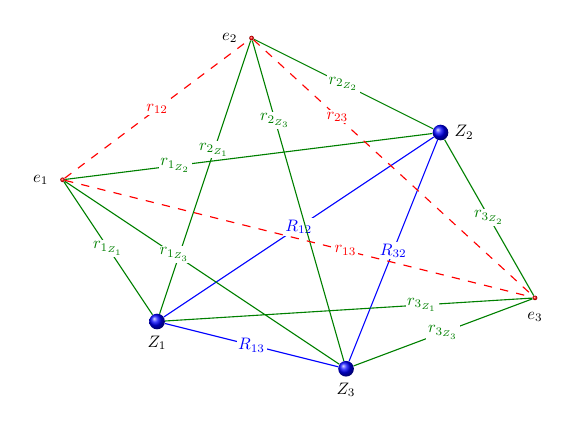
\begin{tikzpicture}[scale=0.6,
						every node/.style={scale=0.6},
						nucleus/.style={ball color=blue, circle},
						electron/.style={ball color=red, circle, inner sep=1pt},
						fw/.style={fill=white, inner sep=1pt},
					]
					\node[nucleus] (Z1) at (-1,0) {}; \node[below=5pt] at (Z1) {$Z_1$};
					\node[nucleus] (Z2) at (5,4) {}; \node[right=5pt] at (Z2) {$Z_2$};
					\node[nucleus] (Z3) at (3,-1) {}; \node[below=5pt] at (Z3) {$Z_3$};

					\node[electron] (e1) at (-3,3) {}; \node[left=5pt] at (e1) {$e_1$};
					\node[electron] (e2) at (1,6) {}; \node[left=5pt] at (e2) {$e_2$};
					\node[electron] (e3) at (7,0.5) {}; \node[below=5pt] at (e3) {$e_3$};

					\draw[blue] (Z1) -- node[fw] {$R_{12}$} (Z2) -- node[fw] {$R_{32}$} (Z3) -- node[fw] {$R_{13}$} (Z1);
					\draw[green!50!black]   (Z1) -- node[fw]            {$r_{1_{Z_1}}$} (e1)
					(Z2) -- node[pos=0.7,fw]      {$r_{1_{Z_2}}$} (e1)
					(Z3) -- node[fw,pos=0.6]            {$r_{1_{Z_3}}$} (e1)
					%
					(Z1) -- node[fw,pos=0.6]           {$r_{2_{Z_1}}$}  (e2)
					(Z2) -- node[fw]          {$r_{2_{Z_2}}$}  (e2)
					(Z3) -- node[fw, pos=0.75] {$r_{2_{Z_3}}$}  (e2)
					%
					(Z1) -- node[fw,pos=0.7]   {$r_{3_{Z_1}}$} (e3)
					(Z2) -- node[fw]           {$r_{3_{Z_2}}$} (e3)
					(Z3) -- node[fw]           {$r_{3_{Z_3}}$} (e3)
					;
					\draw[dashed,red]       (e1) -- node[fw]           {$r_{12}$}     (e2)
					(e1) -- node[fw,pos=0.6]           {$r_{13}$}     (e3)
					(e2) --  node[fw,pos=0.3] {$r_{23}$}     (e3)
					;
				\end{tikzpicture}
			\end{center}
		\end{column}
		\begin{column}{0.4\linewidth}
			\begin{onlyenv}<1>
				\begin{block}{}\footnotesize\justifying
					Квантова хімія розглядає молекулу як утворення з електронів та точкових ядер. Енергія молекули має складові, пов'язані з \emphs{кінетичними енергіями кожного електрона} та \emphs{ядра}, та з \emphs{енергіями їхніх кулонівських взаємодій}.
				\end{block}
			\end{onlyenv}
			\begin{onlyenv}<2>
				\begin{block}{}\footnotesize\justifying
					Життя молекули в квантовій механіці описується її \emphs{хвильовою функцією $\Psi$}. Щоб її знайти --- треба розв'язати стаціонарне \emphs{рівняння Шредінґера} на стани молекулярної системи.
				\end{block}

			\end{onlyenv}
		\end{column}
	\end{columns}
	\begin{onlyenv}<1>
		\begin{multline*}
			\hat{H}_\mathrm{mol} =
			\hat{T}_{n} +
			\hat{T}_{e} +
			{\color{blue} \hat{V}_{nn}} +
			{\color{green!50! black} \tiny \hat{V}_{en}} +
			{\color{red} \hat{V}_{ee}}
			=  - \sum\limits_{\alpha =1}^{K} \frac{1}{2M_{\alpha}} \vec{\nabla}^2_{\alpha}
			-\frac12 \sum\limits_{i}^{N} \vec{\nabla}^2_i  -\\
			{\color{blue}  -\frac12\sum\limits_{\alpha}^{K}\sum\limits_{\beta, \alpha\neq\beta}^{K} \frac{Z_{\alpha}Z_{\beta}}{|\vec{R}_{\alpha}
			- \vec{R}_{\beta}|}}
			{\color{green!50!black} -\sum\limits_{\alpha}^{K}\sum\limits_{i}^{N} \frac{Z_{\alpha}}{|\vec{R}_{\alpha} - \vec{r}_i|}} +
			{\color{red} \frac12 \sum\limits_{i}^{N}\sum\limits_{\substack{j,\, j \neq i}}^{N}\frac{1}{|\vec{r}_i - \vec{r}_j|}}.
		\end{multline*}
	\end{onlyenv}
	\begin{onlyenv}<2>
		\begin{equation*}\label{*}
			\tcbhighmath{\hat{H}_\mathrm{mol} \Psi(\vxi, \vec{R}) = E \Psi(\vxi, \vec{R}),}
		\end{equation*}
		де $\Psi = \Psi(\vxi, \vec{R})$ --- хвильова функція такої системи є функцією координат (як просторових, так і спінових) всіх елек\-тронів  $\vxi = (\vxi_1, \vxi_2, \ldots, \vxi_N)$  та всіх ядер  $\vec{R} = (\vec{R}_1, \vec{R}_2, \ldots, \vec{R}_K)$
	\end{onlyenv}
\end{frame}

%============================================================================





%============================================================================
\begin{frame}{Кінетична енергія ядер --- збурення}{}
	\begin{columns}
		\begin{column}{0.8\linewidth}
			Ядра істотно важче, ніж електрони. Співвідношення між масою протона і електрона:
			\begin{equation*}
				\frac{M}{m} \approx 1836.
			\end{equation*}
		\end{column}
		\begin{column}{0.2\linewidth}
			\begin{center}
				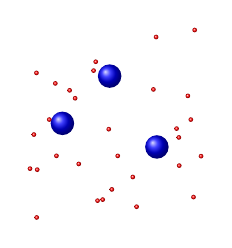
\begin{tikzpicture}[scale=0.6,
						every node/.style={scale=0.6},
						nucleus/.style={ball color=blue, circle, inner sep=5pt},
						electron/.style={ball color=red, circle, inner sep=1pt},
						fw/.style={fill=white, inner sep=1pt},
					]
					\node[nucleus] (Z1) at (-1,0) {};  %\node[below=5pt] at (Z1) {$Z_1$};
					\node[nucleus] (Z2) at (1,-0.5) {};   %\node[right=5pt] at (Z2) {$Z_2$};
					\node[nucleus] (Z3) at (0,1) {};  %\node[below=5pt] at (Z3) {$Z_3$};

					%                    \clip (0,0) circle (4);
					\pgfmathsetseed{4}
					\foreach \p in {1,...,30}
						{ \node[electron] at (2*rand,2*rand) {};}

				\end{tikzpicture}
			\end{center}
		\end{column}
	\end{columns}

	\begin{block}{}
		Існування молекули як єдиного цілого --- рівність імпульсів всіх ядер та електронів \emphz{$p_n = p_e$}, і при суттєвій різниці мас підсистем, їх кінетичні енергії мають суттєво відрізнятись \emphz{$T_n \ll T_e$}, тобто кінетичну енергію ядер $\hat{T}_n$ в гамільтоніані можна вважати \emphs{збуренням} і знехтувати рухом ядер на фоні руху електронної підсистеми.
	\end{block}
\end{frame}
%============================================================================





%============================================================================
\begin{frame}{Електронний гамільтоніан}{}
	Нехтуючи кінетичною енергією ядер  у нас залишився недогризок --- гамільтоніан \alert{електронної підсистеми}:
	\begin{equation*}
		\tcbhighmath{\hat{H}_e(\vec{R}) = \hat{T}_{e} +  \hat{V}_{nn} + \hat{V}_{en} + \hat{V}_{ee},}
	\end{equation*}
	Для такого гамільтоніана сформулювалося електронне рівняння Шредінґера:
	\begin{equation*}
		\tcbhighmath{\hat{H}_e(\vec{R}) \Phi(\vxi\, |\, \vec{R}) = E_e(\vec{R})\Phi(\vxi\,|\,\vec{R})}
	\end{equation*}
	де $\Phi(\vxi|\vec{R})$ --- електронна функція, явно залежить від змінних всіх електронів і визначається при кожному фіксованому положенні ядер.

	\begin{alertblock}{}\small\centering
		Залежність від ядерних змінних як від параметрів підкреслена в запису функції відділенням їх від електронних змінних вертикальної рисою.
	\end{alertblock}

\end{frame}
%============================================================================





%============================================================================
\begin{frame}{Електронна задача}{Квантова хімія}
	Рівняння Шредінґера для електронної задачі:
	\begin{equation*}
		\tcbhighmath{\hat{H}_e(\vec{R})\Phi_m(\vxi\,|\,\vec{R}) = E_{e,m}(\vec{R})\Phi_m(\vxi\,|\,\vec{R})}
	\end{equation*}
	Це рівняння, що визначає стан електронної підсистеми при кожній фіксованій конфігурації ядер, називається електронним рівнянням, а енергія  $E_e(\vec{R})$~--- \emphs{електронним термом молекули}.

	\begin{block}{}\centering
		Власні значення електронного гамільтоніана $E_e(\vec{R})$ --- функції положень ядер!
	\end{block}

	\begin{alertblock}{}\centering
		Пошук розв'язків цієї задачі --- парафія квантової хімії!
	\end{alertblock}
\end{frame}
%============================================================================





%============================================================================
\begin{frame}{Наближення Борна-Оппенгеймера}

	\begin{center}
		Розв'язавши електронну задачу --- переходять до розв'язку ядерної задачі.
	\end{center}

	%    Функції електронної підсистеми --- ортонормовані $\left\langle \Phi_m | \Phi_k \right\rangle = \delta_{mk}.$

	\begin{exampleblock}{}\scriptsize
		Точну функію молекулярної системи можна представити у базисі електронних функцій:
		\begin{equation*}\label{}
			\Psi(\vxi,\vec{R}) = \sum\limits_m^{\infty} \varPsi_m(\vec{R}) \Phi_m(\vxi\,|\,\vec{R}).
		\end{equation*}
		де коефіцієнти розкладання $\varPsi_m(\vec{R})$ --- хвильові функції ядерної підсистеми.

		З фізичної точки зору це означає, що кожному $m$-му стану $\Phi_m(\vxi\,|\,\vec{R})$ електронної підсистеми відповідає свій $m$-й стан $\varPsi_m(\vec{R})$ ядерної підсистеми.
	\end{exampleblock}


	В наближені малості кінетичної енергії ядер (всі можливі електронні стани відповідають лише одній ядерній конфігурації)

	\begin{equation*}\label{}
		\tcbhighmath{\Psi(\vxi,\vec{R}) \approx \varPsi (\vec{R}) \Phi (\vxi\,|\,\vec{R}).}
	\end{equation*}


	%	Рівняння Шредінґера для молекули:
	%
	%	\begin{equation*}
	%		(\hat{T}_n + \hat{H}_e) \varPsi (\vec{R})\Phi (\vxi\,|\,\vec{R}) = {E} \varPsi (\vec{R})\Phi (\vxi\,|\,\vec{R})
	%	\end{equation*}
\end{frame}
%============================================================================





%============================================================================
%\begin{frame}{Ядерна задача}
%	\begin{equation*}
%		(\hat{T} + \hat{H}_e)\sum\limits_m\Phi_m(\varPsi_m(\vec{R})\vxi\,|\,\vec{R}) = {E}\sum\limits_m\varPsi_m(\vec{R})\Phi_m(\vxi\,|\,\vec{R})
%	\end{equation*}
%	Домножимо на $\Phi_k^*(\vxi\,|\,\vec{R})$ і проінтегруємо:
%	\begin{multline*}
%		\underbrace{\sum\limits_m\opbracket{\Phi_k(\vxi\,|\,\vec{R})}{\hat{T} + \hat{H}_e}{\Phi_m(\vxi\,|\,\vec{R})\varPsi_m(\vec{R})}_e}_{\underbrace{\sum\limits_m\opbracket{\Phi_k}{\hat{H}_e}{\varPsi_m\Phi_m}_e}_{E_e\varPsi_k} + \sum\limits_m\opbracket{\Phi_k}{\hat{T}}{\Phi_m\varPsi_m}_e}
%		= \\ =
%		\underbrace{\sum\limits_m\opbracket{\Phi_m(\vxi\,|\,\vec{R})}{E}{\varPsi_k(\vec{R})\Phi_m(\vxi\,|\,\vec{R})}_e}_{E\varPsi_k}
%	\end{multline*}
%    Отримаємо:
%		\begin{equation*}
%			\sum\limits_{m \neq k}\opbracket{\Phi_k}{\hat{T}}{\Phi_m\varPsi_m}_e + \opbracket{\Phi_k}{\hat{T}}{\varPsi_k\Phi_k}_e + E_e\varPsi_k = E\varPsi_k
%		\end{equation*}
%\end{frame}
%============================================================================





%============================================================================
\begin{frame}[t]{Розділення змінних в молекулярному рівнянні}\scriptsize
	Рівняння Шредінґера для молекулярної системи з урахуванням наближення БО:
	\begin{equation*}
		(\hat{T}_n + \hat{H}_e) \varPsi (\vec{R}) \Phi(\vxi\,|\,\vec{R}) = {E}  \varPsi (\vec{R}) \Phi(\vxi\,|\,\vec{R})
	\end{equation*}
	Домножимо на $\Phi^*(\vxi\,|\,\vec{R})$ і проінтегруємо за електронним координатам:
	\begin{equation*}
		\underbrace{\opbracket{\Phi (\vxi\,|\,\vec{R})}{\hat{T}_n + \hat{H}_e}{\varPsi (\vec{R})\Phi(\vxi\,|\,\vec{R})}_e}_{ \opbracket{\Phi}{\hat{T}_n}{\Phi \varPsi }_e + \underbrace{\opbracket{\Phi}{\hat{H}_e}{\varPsi\Phi}_e}_{E_e\varPsi}}
		=
		\underbrace{E \bracket{\Phi_k(\vxi\,|\,\vec{R})}{\varPsi(\vec{R})\Phi(\vxi\,|\,\vec{R})}_e}_{E\varPsi}
	\end{equation*}
	Отримаємо:
	\[
		\opbracket{\Phi}{\hat{T}_n}{\Phi\varPsi}_e + E_e\varPsi = E\varPsi.
	\]
	Розглянемо вираз:
	\[
		\hat{T}_n (\Phi\varPsi) = \Phi\hat{T} \varPsi + (\hat{T} \Phi)\varPsi - \sum\limits_\alpha \frac{1}{M_\alpha}\nabla_\alpha\varPsi\nabla_\alpha\Phi
	\]
	і підставимо в попереднє рівняння
	\begin{equation*}
		\opbracket{\Phi}{\hat{T}}{\varPsi\Phi} =  \underbrace{\bracket{\Phi}{\Phi}}_{=1} \hat{T}\varPsi + \opbracket{\Phi}{\hat{T}}{\Phi}\varPsi   - \frac{1}{M_\alpha} \underbrace{\bracket{\Phi}{\nabla_\alpha\Phi}}_{=0\, \text{в силу}\, \nabla_a \bracket{\Phi}{\Phi} = 0 }\nabla_\alpha\varPsi
	\end{equation*}%
	Інтеграл $\opbracket{\Phi}{\hat{T}_n}{\Phi}_e \approx 0$ у випадку, якщо різниця між сусідніми електронними станами велика $|E_a - E_i| \gg 1$,  тому
	\begin{equation*}
		\left(\hat{T}_n + E_e \right)\varPsi = E\varPsi
	\end{equation*}
\end{frame}
%============================================================================



%============================================================================
%\begin{frame}{Наближення Борна-Оппенгеймера}{Критерії застосування}
%
%        Рівняння для ядерних змінних приймає вигляд
%        \begin{equation*}
%            \left(\hat{T} + E_e \right)\varPsi_k = E\varPsi_k
%        \end{equation*}
%        за умов
%		\begin{align*}
%			\langle  \Phi_k|\nabla_\alpha \Phi_m \rangle = \frac{\opbracket{\Phi_k}{\nabla_\alpha\hat{H}_e}{\Phi_m}}{E_{e,m} - E_{e,k}} \approx 0 \\
%			\langle  \Phi_k|\nabla^2_\alpha \Phi_m \rangle = - \sum\limits_{i\neq k} \frac{\left|\opbracket{\Phi_i}{\nabla_\alpha\hat{H}_e^2}{\Phi_k}\right|^2}{|E_{e,i} - E_{e,k}|^2} \approx 0
%		\end{align*}
%
%\begin{itemize}
%\item  Ці умови виконуються якщо різниця між електронними станами $|E_{e,i} - E_{e,k}|$ велика, тобто \emphs{зміна положень ядер не збурює електронну підсистему}.
%\item 	Чисельник можна інтерпретувати як ймовірність переходу з одного електронного стану $\Phi_i$ до іншого $\Phi_k$.
%\end{itemize}
%
%%	\begin{alertblock}{}
%%		Умова малості цих інтегралів: \alert{ймовірність переходів між електронними станами в результаті зміни положень в ядер в просторі повинні бути незначними.}
%%	\end{alertblock}
%
%\end{frame}
%============================================================================

%============================================================================
\begin{frame}{Ядерна задача}{}
	Рівняння для ядерних хвильових функцій $\varPsi(\vec{R})$:
	\begin{equation*}\label{}
		\tcbhighmath{\left(\hat{T}(\vec{R}) + E_{e,k}(\vec{R}) \right)\varPsi(\vec{R})
			= E\varPsi(\vec{R})}
	\end{equation*}

	Гамільтоніан наближення \emphz{$\hat{H}_\mathrm{BO} = \hat{T}(\vec{R}) + E_{e}(\vec{R})$}
	визначає рух ядерної підсистеми під дією електронів. Складається з кінетичної енергії ядер $\hat{T}(\vec{R})$ і ефективного потенціалу $E_{e}(\vec{R})$, який створюють електрони.


	\begin{block}{}\scriptsize\justifying
		Все внутрішнє <<копирсання>> електронів, вся кулонівська кухня, для ядер накрита <<килимом>>: ядра відчувають лише деяку поверхню потенціальної енергії (ППЕ) $E_{e}(\vec{R})$, а
		звідки вона береться --- вони навіть не в курсі.
	\end{block}

	\begin{block}{}\scriptsize\justifying
		Для електронів картина інша: вони настільки швидкі, що бачать лише великі ядра, які стоять на місці і приймають деякий стаціонарний стан. При зміщеннях ядер, електрони швидко приймають найбільш вигідне положення, не змінюючи свій стан.
	\end{block}
\end{frame}
%============================================================================






%============================================================================
\begin{frame}[t]{Поверхня потенціальної енергії}{}
	%---------------------------------------------------------
	\begin{onlyenv}<1>
		Графічний вигляд цієї гіперповерхні $E_\mathrm{e}(\vec{R})$ з конфігураційному просторі $3K$ координат називається \emphs{поверхнею потенціальної енергії (ППЕ)} молекули.
	\end{onlyenv}
	\begin{onlyenv}<2>
		\emphs{Внутрішні координати $q_i$} --- набір усіх довжин зв'язків, валентних кутів та торсіонних кутів.  Число внутрішніх координат $3K - 6$ (а для лінійних молекул $3K - 5$).
	\end{onlyenv}
	\begin{onlyenv}<3>
		Тип стаціонарної точки визначається матрицею других похідних, яка називається матрицею Гессе.
	\end{onlyenv}
	\begin{onlyenv}<4>
		Структура молекули --- \emphs{локальний} або \emphs{глобальний мінімум} на ППЕ. Пошук мінімуму --- \emphs{оптимізація структури молекули}.
	\end{onlyenv}
	\begin{onlyenv}<5>
		За фізичним змістом матриця Гессе ---  є \emphs{матрицею силових констант молекули}.
	\end{onlyenv}
	\begin{columns}
		\begin{column}{0.6\linewidth}
			\begin{onlyenv}<1>
				\begin{block}{}
					Геометричний образ цієї поверхні в багатовимірному просторі, що визначають ядерну конфігурацію, побудувати не можна, однак можна розглядати окремі перерізи або проекції на ту чи іншу координатну площину.
				\end{block}
			\end{onlyenv}
			\framesubtitle<2>{Теорема Гельмана-Фейнмана. Внутрішні координати молекули}
			\begin{onlyenv}<2>
				\begin{equation*}
					\tcbhighmath{F_i = \frac{\partial E}{\partial q_i} = \opbracket{\Phi}{\frac{\partial \hat{H}}{\partial q_i}}{\Phi}}
				\end{equation*}
				\begin{itemize}\small
					\item  Точки в ядерному конфігураційному просторі, де $F_i = 0$, для всіх ядер --- \emphs{стаціонарні точки} на ППЕ.
					\item Сили, що діють на ядро в молекулі, є точно класичними електростатичними силами, що виникають із-за взаємодії зарядів ядер та електронів (\emphs{електро\-статична теорема}).
				\end{itemize}
			\end{onlyenv}
			\framesubtitle<3>{Матриця Гессе --- матриця кривизни ППЕ}
			\framesubtitle<5>{Матриця Гессе --- матриця силових констант молекули}
			\begin{onlyenv}<3>
				\begin{equation*}\label{}
					\begin{bmatrix}
						\dfrac{\partial^2 E_e}{\partial q_1^2}             & \dfrac{\partial^2 E_e}{\partial q_1\,\partial q_2} & \cdots & \dfrac{\partial^2 E_e}{\partial q_1\,\partial q_n} \\
						\dfrac{\partial^2 E_e}{\partial q_2\,\partial q_1} & \dfrac{\partial^2 E_e}{\partial q_2^2}             & \cdots & \dfrac{\partial^2 E_e}{\partial q_2\,\partial q_n} \\
						\vdots                                             & \vdots                                             & \ddots & \vdots                                             \\
						\dfrac{\partial^2 E_e}{\partial q_n\,\partial q_1} & \dfrac{\partial^2 E_e}{\partial q_n\,\partial q_2} & \cdots & \dfrac{\partial^2 E_e}{\partial q_n^2}
					\end{bmatrix}
				\end{equation*}
			\end{onlyenv}
			\begin{onlyenv}<5>
				\begin{equation*}\label{}
					\begin{bmatrix}
						\dfrac{\partial^2 E_e}{\partial q_1^2} & 0                                      & \cdots & 0                                      \\
						0                                      & \dfrac{\partial^2 E_e}{\partial q_2^2} & 0      & 0                                      \\
						\vdots                                 & \vdots                                 & \ddots & \vdots                                 \\
						0                                      & 0                                      & \cdots & \dfrac{\partial^2 E_e}{\partial q_n^2}
					\end{bmatrix}
				\end{equation*}
			\end{onlyenv}
			\framesubtitle<4>{Оптимізація структури молекули}
			\begin{onlyenv}<4>
				\noindent%
				\begin{block}{}\justifying
					Мінімуми на ППЕ відповідають рівноважним міжядерним відстаням (довжини хімічних зв'язків), певним валентним і двогранним кутам, які в свою чергу характеризують \emphs{молекулярну структуру} --- геометричний образ, що використовується при описі будови молекули в класичній механіці.
				\end{block}
				%Саме в квантовій механіці молекулярна структура стає цілком визначеним поняттям тільки в наближенні Борна-Оппенгеймера, і як це не дивно, саме це наближення дозволяє нам мати наочний образ молекули.
			\end{onlyenv}
		\end{column}%
		%---------------------------------------------------------
		\begin{column}{0.4\linewidth}\centering
			\begin{onlyenv}<1,3,4>\centering
				\includegraphics[width=1\linewidth]{ppe}
			\end{onlyenv}
			\begin{onlyenv}<2>\centering
				\includegraphics[width=0.75\linewidth]{MolCoord}
			\end{onlyenv}
			\begin{onlyenv}<5>
				\hspace*{-2.5em}
				%				\begin{center}
				\begin{tikzpicture}[scale=2, >=latex]
					\message{^^JMorse potential}
					\def\xmax{2} % max x axis
					\def\A{1}
					\def\b{3.3}
					\def\a{(0.26*\xmax)}

					\def\ymax{1.50}  % max y axis
					\draw[->,thick] (0,-0.1*\ymax) -- (0,1.1*\ymax) node[right] {$E_e$};
					\draw[->,thick] (-0.1*\ymax,0) -- (1.2*\xmax,0) node[below, pos=0.6, font=\tiny] {Міжмолекулярна відстань};
					\draw[red, samples=100,smooth, name path=parabola, variable=\x,domain=0.34*\a:1.66*\a]     plot(\x,{\A*\b^2*(\x-\a)^2});
					\foreach \i[count=\j] in {0.1,0.2,...,1}%
						{
							\path[name path={E\j}] (0, \i) -- ({1.2*\xmax},\i);
							\draw[red,name intersections={of={E\j} and parabola}] (intersection-1) -- (intersection-2);
						}
					\node[below] at ({\a}, 0) {$R_0$};
					\draw[blue, name path=morse, samples=100,smooth,variable=\x,domain=0.145*\xmax:1.2*\xmax]
					plot(\x,{\A*(1-exp(-\b*(\x-\a)))^2});
					\foreach \i[count=\j from 0] in {0.12,0.24,0.36,...,0.92}%
						{
							\path[name path={E\j}] (0, \i) -- ({1.2*\xmax},\i);
							\draw[blue,name intersections={of={E\j} and morse}] (intersection-1) -- (intersection-2) node[right, font=\tiny, black] {$n = \j$};
						}
					\draw[dashed] (0, {\A+0.05}) -- (1.2*\xmax, {\A+0.05}) node[above, font=\tiny, pos=0.6] {Дисоціаційна межа};
					\node[atom] (A) at ({\a - \a/3}, {0.95*\ymax}) {};
					\node[atom] (B) at ({\a + \a/3}, {0.95*\ymax}) {};
					\draw[boundH] (A) -- node[above] {} (B);
				\end{tikzpicture}
				%				\end{center}
			\end{onlyenv}
		\end{column}
		%---------------------------------------------------------
	\end{columns}
	\begin{onlyenv}<3>\footnotesize
		\vspace*{-1em}
		\begin{itemize}
			\item \emphs{локальні мінімуми} на потенціальної поверхні --- відповідають метастабільним конфігураціям молекули.
			\item \emphs{абсолютний мінімум} --- найстійкішою (стабільною) конфігурацією --- основного стану системи.
			\item \emphs{сідлові точки} --- відповідають перехідним станам.
		\end{itemize}
	\end{onlyenv}
	\begin{onlyenv}<4>\centering
		Початкова геометрія молекули може бути вибрана на основі хімічних міркувань.	\end{onlyenv}
	\begin{onlyenv}<5>
		У гармонічному наближенні компоненти діагоналізовної матриці в точці мінімуму визначають \emphs{енергії} і \emphs{власні частоти коливань ядер}:
		\begin{equation*}
			E_n = \left(n + \frac12\right) \hbar \omega
		\end{equation*}
	\end{onlyenv}
\end{frame}
%============================================================================






%============================================================================
\begin{frame}[t]{Що не описується наближенням БО?}{}
	%---------------------------------------------------------

	\framesubtitle<1>{Вібронний зв'язок в молекулі}
	\begin{onlyenv}<1>
		Якщо енергія ядерних коливань порівнянна з різницею енергій основного та збуджених електронних станів --- виникають \emphs{вібронні стани}, які залежать від взаємодії електронної та ядерної підсистем: \emphs[red]{адіабатичний потенціал втрачає свій фізичний сенс}, електронний рух невід'ємний від ядерного.
		\begin{columns}
			\begin{column}{0.55\linewidth}
				\begin{itemize}\footnotesize
					%					\item При вібронному переході відбувається одночасна зміна електронних і ядерних коливальних рівнів енергії молекули в результаті поглинання або випускання фотона відповідної енергії.
					\item \emphs{Принцип Франка-Кондона} --- при електронних переходах положення атомів фіксовані (вертикальний перехід). Після переходу геометрія молекули релаксує.
					\item \href{https://en.wikipedia.org/wiki/Jahn\%E2\%80\%93Teller_effect}{\emphs{Ефекти Яна-Теллера}} --- зниження симетрії ядерної конфігурації при виродженій хвильовій функції електронної підсистеми, що проявляється у геометричному спотворенні молекул.
				\end{itemize}
			\end{column}
			\begin{column}{0.45\linewidth}
				\includegraphics[width=\linewidth]{Vibron}
			\end{column}
		\end{columns}
	\end{onlyenv}
	% -------------------------------------
	\framesubtitle<2>{Ефект Яна-Теллера --- конічний перетин}
	\begin{onlyenv}<2>
		\href{https://ru.qaz.wiki/wiki/Conical_intersection}{\emphs{Конічний перетин}} --- це перетин двох або більшого числа потенціальних енергетичних поверхонь. Кореловані рух електронів і коливання ядер можуть призвести до спотворення конфігурації та зниження симетрії, при цьому виродження знімається, а поверхня потенційної енергії розщеплюється на дві.
		\begin{columns}
			\begin{column}{0.6\linewidth}
				\begin{itemize}\scriptsize
					\item Після поглинання фотона геометрія молекули поступово змінюється у напрямку до мінімуму на ППЕ збудженого стану;
					\item Через конічний перетин відбувається перехід з ППЕ збудженого стану на ППЕ основного;
					\item Геометрія молекули поступово змінюється у напрямку до мінімума на ППЕ основного стану (утворюється цис- або транс-ізомери).
				\end{itemize}
			\end{column}
			\begin{column}{0.4\linewidth}
				\includegraphics[width=1\linewidth]{CiS-Trans}
			\end{column}
		\end{columns}
		\begin{block}{}\scriptsize
			Конічні перетини також називають \emphs[red]{молекулярними лійками} або \emphs[red]{диявольськими точками}, оскільки вони стали усталеною парадигмою для розуміння механізмів реакцій в фотохімії, настільки ж важливі, як перехідні стани в термічній хімії.
		\end{block}
	\end{onlyenv}
\end{frame}
%============================================================================




%============================================================================
\begin{frame}{Висновки}{}
	\begin{enumerate}[\faHandORight]
		\item Поняття структури молекули можливе лише в рамках наближення Борна-Оппенгеймера.
		\item Наближення дозволяє розділити змінні в молекулярному гамільтоніані і, як наслідок, розділити молекулярну систему на електронну та ядерну підсистеми.
		\item Енергія електронної підсистеми є потенціалом для ядерної підсистеми.
		\item Геометричний образ функції енергії електронної підсистеми є гіперповерхнею в конфігураційному просторі ядерних координат. Характеристики цієї поверхні дозволяють обчислювати властивості молекули.
		\item Наближення несправедливе якщо енергія ядерних коливань співмірна з різницею енергій основного і збудженого електронних станів.
	\end{enumerate}
\end{frame}
%============================================================================





%============================================================================
\end{document}
